\documentclass[11pt]{article}

\usepackage[bookmarks=true]{hyperref}
\usepackage[a4paper,margin=2.5cm]{geometry}
\usepackage[fleqn]{amsmath}
\usepackage{graphicx}

\usepackage{amsthm}
\usepackage{amssymb}
\usepackage{stmaryrd}
\usepackage{amsfonts}
\usepackage{etoolbox}
\usepackage{enumerate}
\usepackage{scalerel}
\usepackage{stackengine}
\usepackage{xifthen}
\usepackage{lmodern}
\usepackage{gensymb}
\usepackage{color}
\usepackage{colortbl}
\usepackage{needspace}
\usepackage{enumitem}
\usepackage{mathtools}
\usepackage{bbm}
\usepackage{xargs}
\usepackage{algorithm}
\usepackage{diagbox}
\usepackage{subcaption}
\usepackage[table]{xcolor}
\usepackage[noend]{algpseudocode}
\usepackage{polynom}

\newcommand{\naturals}{\mathbb{N}}
\newcommand{\integers}{\mathbb{Z}}
\newcommand{\reals}{\mathbb{R}}
\newcommand{\complex}{\mathbb{C}}
\newcommand{\rationals}{\mathbb{Q}}

\DeclarePairedDelimiterX{\set}[1]\lbrace\rbrace{\setaux #1||\endsetaux}
\def\setaux#1|#2|#3\endsetaux{\if\relax\detokenize{#2}\relax #1 \else #1 \;\delimsize\vert\; #2 \fi}

% Q.E.D.
\renewcommand{\qedsymbol}{\footnotesize$\boxempty$ \textsc{q.\,e.\,d.}}


\theoremstyle{definition}
\newtheorem{fact}{Fact}
\newtheorem{conjecture}{Conjecture}
\newtheorem{theorem}{Theorem}
\newtheorem{lemma}{Lemma}
\newtheorem{claim}{Claim}

\title{Experiments and analysis for selected robust network design problem classes}
\author{David Dekker \\ \texttt{d.j.c.dekker@student.tue.nl} \and Sten Wessel \\ \texttt{s.wessel@student.tue.nl}}
\date{\today}

% Document
\begin{document}
    \maketitle
    \hrule
    \bigskip

    \section{Introduction} \label{sec:introduction}
    We consider a graph $G = (V, E)$ with a set of terminals $W \subseteq V$, together with a set of valid traffic demands between terminals represented by a matrix $(D_{ij})_{i,j \in W}$.
    We refer to the set of valid demands as the \emph{demand universe} $\mathcal U$.
    The goal in robust network design is to construct a network on $G$ by buying capacities on the edges such that every valid traffic demand can be routed on the network.
    The usual challenge is to minimize the cost of the network, defined by $\sum_{e \in E} c_e x_e$, where $x_e$ denotes the bought capacity for edge $e$, and $c_e$ the per-unit-capacity cost of the edge.

    Although the network needs to be able to route multiple demand matrices, we disallow changing the routing paths between terminals if demands change.
    This is referred to the \emph{oblivious} routing model, where each pair of terminals $i,j \in W$ has a fixed routing path $P_{ij}$ for all routing all demands.
    Hence, for every edge $e$ on the path $P_{ij}$ we must buy a capacity of at least $D_{ij}$, for each demand matrix $D \in \mathcal U$.
    We refer to the set of paths $\mathcal P = \set{P_{ij} : i,j \in W}$ as the \emph{routing template}.
    The routing template, together with the bought capacities for the edges, forms the solution to a robust network design problem.

    Robust network design has been studied on specific classes of demand universes.
    Such as special class are the \emph{hose matrices} $\mathcal H = \set{(D_{ij}) : \sum_j D_{ij} \le b_i \quad \forall_{i \in W}}$, where $b_i$ denotes the \emph{marginal} demand for terminal $i$, that describes the maximum amount of traffic communicated from this terminal.
    The demands are viewed as undirected, hence $D_{ij} = D_{ji}$ describes the single demand between $i,j$.
    Designing a minimum cost network for the class of hose matrices is known as the \emph{virtual private network (VPN) problem}.
    A $2$-approximation algorithm for the VPN problem was shown both in \cite{fingerhut1997designing} and \cite{gupta2001provisioning}.
    It was conjectured \cite{italiano2006design} that this algorithm is in fact optimal.
    The conjecture was initially shown to hold on ring networks (the constrained setting where $G$ is a cycle) and some other special cases~\cite{hurkens2007virtual}, and was later resolved for arbitrary networks as well~\cite{goyal2013vpn}.

    In this report, we consider two additional classes of (polyhedral) demand universes.
    We first look into \emph{tree demands}, generalizing the class of hose matrices.
    The robust network design problem for tree demands is known as the \emph{generalized VPN problem}.
    The 2-approximation algorithm for the VPN problem has a natural extension to the generalized case, and it is conjectured that this algorithm is optimal in this setting as well \cite{OLVER2016191}.
    However, this remains unresolved.
    In this report, we discuss this algorithm and discuss some efforts of proving the conjecture on ring networks.

    % TODO: introduction capped hose.

    % TODO: V_G E_G and binom W 2

    \section{Generalized VPN problem}
To describe the generalized VPN problem, we first describe the class of tree demands.
Let $G = (V_G, E_G)$ be the underlying network graph with terminal set $W \subseteq V_G$.
Let an edge-capacitated tree $T = (V_T, E_T)$ be given with leaf set exactly the terminals $W$, and edge capacities $b_e$ for $e \in E_T$.
Then $T$ describes the tree demand universe $\mathcal U_T$ where a symmetric demand matrix $(D_{ij})$ belongs to $\mathcal U_T$ when it can be routed on $T$.
That is, for all edges $e$ on the (unique) path $\pi_T(i,j)$ between $i$ and $j$ in $T$ it must hold that $D_{ij} \le b_e$.
Note that if we take $T$ to be a star with center $r$ and edge capacities $b_{ir} = b_i$, then $\mathcal U_T$ describes the same universe as the hose model $\mathcal H$ with marginal demands $b_i$.
Hence, tree demands indeed generalize the hose model.

The generalized VPN is now fully characterized by the underlying network graph $G$, a terminal set $W$, edge per-unit-capacity costs $c_e$ ($e \in E_G$), and the \emph{demand tree} $T$ with edge capacities $b_f$ ($f \in E_T$).
A solution to the problem consists of a routing template $\mathcal P = \set{P_{ij} : i,j \in \binom W 2}$ and bought edge capacities $x_e$ for all $e \in E_G$.
We call a solution \emph{feasible} when all demand matrices in $\mathcal U_T$ can be routed on $G$ according to the routing template and without exceeding the installed edge capacities $x$.
We furthermore call a solution optimal if it is feasible and minimizes $\sum_{e \in E_G} c_e x_e$.

\subsection{Integer programming formulation}
The generalized VPN problem can be formulated as the integer program~\eqref{eq:gvpn:mip:semiinf:obj}--\eqref{eq:gvpn:mip:semiinf:f}.
\begin{alignat}{5}
    \text{minimize}\ && \sum_{uv \in E_G} c_{uv} \cdot x_{uv} &&& \label{eq:gvpn:mip:semiinf:obj}\\
    \text{subject to}\ && x_{uv} &\ge \sum_{ij \in \binom{W}{2}} D_{ij} \cdot (f_{uv}^{ij} + f_{vu}^{ij}) &&\qquad \forall_{uv \in E_G,\ D \in \mathcal U_T} \label{eq:gvpn:mip:semiinf:demand}\\
    && \sum_{uv \in \delta(u)} (f_{uv}^{ij} - f_{vu}^{ij}) &= \begin{cases}
                                                                  1 & \text{if $u = i$} \\
                                                                  -1 & \text{if $u = j$} \\
                                                                  0 & \text{otherwise}
    \end{cases} &&\qquad \forall_{u \in V_G,\ ij \in \binom{W}{2}} \label{eq:gvpn:mip:semiinf:flow}\\
    && x_{uv} &\in \mathbb{R}_+ &&\qquad \forall_{uv \in E_G} \label{eq:gvpn:mip:semiinf:x}\\
    && f_{uv}^{ij},\ f_{vu}^{ij} &\in \{ 0, 1 \} &&\qquad \forall_{uv \in E_G,\ ij \in \binom{W}{2}} \label{eq:gvpn:mip:semiinf:f}
\end{alignat}
Each edge $uv$ has constant cost $c_{uv}$ and has a non-negative variable $x_{uv}$ indicating the bought capacity for this edge.
The objective is then to minimize the total cost, i.e.\ the sum of $c_{uv} x_{uv}$ over all edges $uv$.

For each unordered pair of terminals $\set{i, j} \in \binom W 2$, a routing path between these terminals is constructed using binary flow variables.
The flow variable $f_{uv}^{ij}$ indicates whether the directed edge $(u, v)$ is used on the path from terminal $i$ to $j$.
This can be modeled with traditional flow constraints in constraint~\eqref{eq:gvpn:mip:semiinf:flow}.
The routing path from $i$ to $j$ is then given by the set of directed edges $\set{(u, v) \in E_G | f_{uv}^{ij} = 1}$.
By symmetry, we only need to consider one ordering of all unordered pairs.
For ease of notation, we will still describe flow variables with $f_{uv}^{ij}$.

Constraint~\eqref{eq:gvpn:mip:semiinf:demand} ensures that we buy enough capacity on each edge.
For a demand matrix $D \in \mathcal U_T$, we can derive the required capacity on an edge $uv$ using the flow variables.
If $f^{ij}_{uv}$ or $f^{ij}_{vu}$ is 1, then we must buy $D_{ij}$ capacity on edge $uv$ to facilitate the flow between terminals $i$ and $j$.
Thus, we obtain the constraint
\[
    x_{uv} \ge \sum_{ij \in \binom W 2} D_{ij} ( f^{ij}_{uv} + f^{ij}_{vu}),
\]
which must hold for any edge $uv$ and for any demand matrix $D_{ij} \in \mathcal U_T$.

This definition leads to an infinite number of constraints as $\mathcal U_T$ is in general not a finite set of matrices.
This issue can be resolved with row generation, where we solve the program by only considering a subset $\mathcal U_T^* \subset \mathcal U_T$ in constraint~\eqref{eq:gvpn:mip:semiinf:demand}.
Then we obtain a solution $(\tilde x, \tilde f)$ that is only valid for all $D \in \mathcal U_T^*$.
We then assess whether there exists a matrix $D \in \mathcal U_T \setminus \mathcal U_T^*$ that violates the constraint.
If such a matrix exists, we add it to $\mathcal U_T^*$ and solve the program again until we cannot find any violating matrix.
Note that a violating matrix $D$ satisfies
\[
    \tilde x_{uv} < \sum_{ij \in \binom W 2} D_{ij} \cdot (\tilde f^{ij}_{uv} + \tilde f^{ij}_{vu})
\]
for some edge $uv \in E_G$.
We can thus find such a violating matrix by solving the following linear subproblems, one for each $uv \in E_G$:
\begin{alignat*}{5}
    p_{uv} = \text{maximize}\quad && \sum_{ij \in \binom{W}{2}} (\tilde f_{uv}^{ij} + \tilde f_{vu}^{ij}) \cdot D_{ij} &&& \\
    \text{subject to}\quad && \sum_{\substack{ij \in \binom{W}{2}\\e \in \pi_T(i,j)}} D_{ij} &\le b_e &&\qquad \forall_{e \in E_T} \\
    && D_{ij} &\in \mathbb{R}_+ &&\qquad \forall_{ij \in \binom{W}{2}}
\end{alignat*}
If for any of these subproblems the optimal solution $D^*$ has objective $p_{uv} > \tilde x_{uv}$, we add $D^*$ to $\mathcal U_T^*$.
Otherwise, $\mathcal U_T^*$ was representative for $\mathcal U_T$ and we can conclude that the integer program~\eqref{eq:gvpn:mip:semiinf:obj}--\eqref{eq:gvpn:mip:semiinf:f} is optimal.

Although the row generation subproblems do not contain integer variables, the overall procedure to find an optimal solution for \eqref{eq:gvpn:mip:semiinf:obj}--\eqref{eq:gvpn:mip:semiinf:f} may use a large number of iterations.
Using a clever dualization trick (also performed in~\cite{altin2007provisioning}) we can obtain a compact MIP formulation that does not require row generation.

For this trick, consider a single edge $uv \in E_G$ and consider $f$ as parameters.
Note that we can write constraint~\ref{eq:gvpn:mip:semiinf:demand} as
\[
    x_{uv} \ge \max_{D \in \mathcal U_T} \sum_{ij \in \binom W 2} D_{ij} \cdot (f^{ij}_{uv} + f^{ij}_{vu}),
\]
or, when writing out the polyhedral constraints describing $\mathcal U_T$, as the optimization problem
\begin{alignat}{5}
    x_{uv} \ge \text{maximize}\ && \sum_{ij \in \binom{W}{2}} (f_{uv}^{ij} + f_{vu}^{ij}) \cdot D_{ij} &&& \\
    \text{subject to}\ && \sum_{\substack{ij \in \binom{W}{2}\\e \in \pi_T(i,j)}} D_{ij} &\le b_e &&\qquad \forall_{e \in E_T} \label{eq:gvpn:dualtrick} \\
    && D_{ij} &\in \mathbb{R}_+ &&\qquad \forall_{ij \in \binom{W}{2}}
\end{alignat}
Since this linear program is feasible and bounded, we might just as well write the dual
\begin{alignat}{5}
    x_{uv} \ge \text{minimize}\ && \sum_{e \in E_T} b_e \cdot \omega_e^{uv} &&& \label{eq:gvpn:dualtrick:min} \\
    \text{subject to}\ && \sum_{e \in \pi_T(i,j)} \omega_e^{uv} &\ge f_{uv}^{ij} + f_{vu}^{ij} &&\qquad \forall_{ij \in \binom{W}{2}} \\
    && \omega_e^{uv} &\in \mathbb{R}_+ &&\qquad \forall_{e \in E_T}
\end{alignat}
where $\omega_e^{uv}$ are the  dual variables for constraint~\ref{eq:gvpn:dualtrick}.
Now, note that we can drop the minimize in \ref{eq:gvpn:dualtrick:min} as the objective function of the original MIP is a non-negatively weighted sum of the variables $x_{uv}$.
We now have thus obtained a compact MIP formulation for the generalized VPN problem:
\begin{alignat*}{5}
    \text{minimize}\ && \sum_{uv \in E_G} c_{uv} \cdot x_{uv} &&& \\
    \text{subject to}\ && x_{uv} &\ge \sum_{e \in E_T} b_e \cdot \omega_e^{uv} &&\qquad \forall_{uv \in E_G} \\
    && \sum_{e \in \pi_T(i,j)} \omega_e^{uv} &\ge f_{uv}^{ij} + f_{vu}^{ij} &&\qquad \forall_{uv \in E_G,\ ij \in \binom{W}{2}} \\
    && \sum_{uv \in \delta(u)} (f_{uv}^{ij} - f_{vu}^{ij}) &= \begin{cases}
                                                                1 & \text{if $u = i$} \\
                                                                -1 & \text{if $u = j$} \\
                                                                0 & \text{otherwise}
    \end{cases} &&\qquad \forall_{u \in V_G,\ ij \in \binom{W}{2}} \\
    && x_{uv} &\in \mathbb{R}_+ &&\qquad \forall_{uv \in E_G} \\
    && \omega_e^{uv} &\in \mathbb{R}_+ &&\qquad \forall_{uv \in E_G,\ e \in E_T} \\
    && f_{uv}^{ij},\ f_{vu}^{ij} &\in \{ 0, 1 \} &&\qquad \forall_{uv \in E_G,\ ij \in \binom{W}{2}}
\end{alignat*}

\subsection{Hierarchical hubbing algorithm}
\begin{algorithm}
    \caption{RecursiveHubbing}
    \label{alg:TriangulateStar}
    \begin{algorithmic}[1]
        \Statex Recursive enumeration algorithm to find all optimal mappings. Initially, verticesToAssign equals $V_T - W$ and $h$ is an empty mapping from $V_T$ to $V_G$. In the actual implementation, we also maintain a set of all best mappings that attain the minimum cost.

        \Procedure{Assign}{verticesToAssign, $h$}
            \If {verticesToAssign is empty}
                \State \Return $\sum_{uv \in E_T} d(h(u), h(v))$ \Comment{The cost of mapping $h$}
            \EndIf

            \State $u \gets$ verticesToAssign.first()
            \State bestCost $\gets \infty$

            \ForAll {vertices $v$ in graph}
                \State $h(u) \gets v$
                \State currentCost $\gets$ \textsc{Assign}(verticesToAssign $-$ $u$, $h$)

                \If {currentCost $<$ bestCost}
                    \State bestCost $\gets$ currentCost
                \EndIf
            \EndFor

            \State \Return bestCost
        \EndProcedure
    \end{algorithmic}
\end{algorithm}

TODO ref suggested an 8-approximation algorithm for this problem. %TODO ref
They considered the optimal solution over all \emph{hubbing solutions}.
A hubbing solution maps each internal node in the demand tree to a vertex in $V_G$.
Each terminal must be mapped to its corresponding vertex in $G$.
This mapping function is denoted with $h$
For each edge $uv$ in the demand tree, we then buy $b_{uv}$ capacity along the shortest path between $h(u)$ and $h(v)$ in the original graph $G$, where each edge $e$ has its cost $c_e$ as weight.
The total cost then becomes
\[
    \sum_{uv \in E_T} b_{uv} d_c(h(u), h(v)),
\]
where $d_c(h(u), h(v))$ gives the distance between $h(u)$ and $h(v)$ in $G$ where $c$ defines the edge weights.
It was conjectured that this algorithm is optimal, i.e.\ that an optimal hubbing solution is an optimal solution for the generalized VPN problem.

Algorithm~\ref{alg:TriangulateStar} describes a recursive algorithm to find the optimal hubbing solution.
With a standard recursive approach, the total cost is calculated for each mapping $h$ from $V_T \setminus W$ to $V_G$.
The optimal cost is then returned; notice that the actual mapping can easily be returned as well.
From this mapping, the routing templates can be derived.

However, it is possible to determine the optimal hubbing solution more efficiently using dynamic programming. %TODO ref
We first pick an arbitrary internal node of the demand tree as root.
Then we root the demand tree here.
A subtree of this tree is a tree that is rooted at a vertex in this tree, i.e.\ a vertex and all nodes below it.
This tree has a parent (unless it is the entire tree) and children (unless the root is a terminal).
Algorithm~\ref{alg:subtrees} derives the set of subtrees, denoted by $\mathcal L$, in a BFS manner.

For any subtree $S \in \mathcal L$ and vertex $v \in V_G$, we consider the subproblem $C[S, v]$.
It stores the cost of an optimal hubbing solution of the problem restricted to subtree $S$, where the root of $S$ is mapped to $v$.
The final solution is then $\min_{v \in V_G} C[T, v]$.

Let $S_w$ denote the subtree rooted at a vertex $w \in T$.
Now suppose that we want to obtain the value for $C[S_r, v]$ for some vertex $r \in V_T$ and $v \in V_G$, while $C[S_{r_i}, w]$ is known for all children $r_i$ of $r$ and all vertices $w \in V_G$.
Then the mappings of the subtrees are independent of each other.
The contribution of one specific subtree $S_{r_i}$ to the cost of subtree $S_r$ is
\[
    \min_{w \in V_G} \left( C[S_{r_i}, w] + b_{r, r_i} d_c(v, w) \right).
\]
Notice that the mapping of $r$ is $v$ and the mapping of $r_i$ is $w$ in this recurrence.
We minimize the cost of this subtree over all possible choices for $w$.
This gives the following recurrence.
\[
    C[S_r, v] = \begin{cases}
                  0 &\text{if $r \in W$ and $r = v$} \\
                  \infty &\text{if $r \in W$ and $r \neq v$} \\
                  \displaystyle \sum_{\text{children $r_i$ of $r$}} \min_{w \in V_G} \Big( C[S_{r_i}, w] + b_{r, r_i} d(v, w) \Big) &\text{otherwise} \\
    \end{cases}
\]

\begin{algorithm}
    \caption{Finding all subtrees for the dynamic programming algorithm}
    \label{alg:subtrees}
    \begin{algorithmic}[1]
        \Statex Obtaining all subtrees that are needed for the dynamic programming algorithm.
        The dynamic program itself only fills in the table based on the recurrence stated below.
        \Procedure{GetSubtrees}{$V_T, E_T, W$}
            \State root = arbitrary node in $V_T - W$

            \State $\mathcal L \gets \emptyset$
            \State $S \gets$ Subtree(root, root.neighbors, null) \Comment{A subtree has a root, children and parent}
            \State $\mathcal L$.add($S$)
            \State $\mathcal Q$.add($S$)

            \While {$\mathcal Q$ is not empty}
                \State tree = $\mathcal Q$.removeFirst
                \State currentRoot $\gets$ tree.root
                \ForAll{vertices $r$ in tree.children}
                    \State $S$ = Subtree($r$, $r$.neighbors $-$ currentRoot, currentRoot)
                    \State $\mathcal L$.add($S$)
                    \State $\mathcal Q$.add($S$)
                \EndFor
            \EndWhile
            \State \Return subtrees.reversed()
        \EndProcedure
    \end{algorithmic}
\end{algorithm}

\subsection{Experiments}
All the experiments we have seen.
Integrality gap results.

\subsection{Ring networks}
The paper by Grandoni et al.~\cite{grandoni2008short} gives a short proof that the VPN conjecture is true for the cases where the considered network is a ring.
In the following, we will discuss whether it is possible to extend the proof to the generalized VPN conjecture, for the cases where the network is a ring and the demand tree is a \emph{two-union star}: the tree formed by connecting the centers of two star graphs.

Some background of what steps we are taking is identical to what is described in \cite{grandoni2008short} and we will omit these details.
We focus on showing the differences that are necessary in the proof to adapt to the generalized VPN problem setting.
We use the same notation as used in the aforementioned paper, except where the generalized VPN problem differs from the VPN problem.

For the remainder, we restrict ourselves to instances where $T$ is a \emph{two-union star}, that is, a tree formed by connecting the centers $r_1,\ r_2$ of two star graphs.
We will call this edge $r = \set{r_1, r_2}$ and refer to it as the \emph{bridge} of $T$.

\subsubsection{Preliminaries}
A number of assumptions are made in \cite{grandoni2008short}, the most important being that we can assume the capacities $b \equiv 1$.
We suspect this does not quite generalize to our case, but we can state the following:

\begin{fact}
    We may assume $b(f) = 1$ when $f \neq r$.
\end{fact}
Using the same motivation as in \cite{grandoni2008short}, if the capacity $b(iu)$ for the terminal $i \in W$ is not unit, construct a new instance with new terminals $i_1, \dots, i_{b(iu)}$, connected to the site of $i$ in $G$, with edge cost $0$.
Set the capacities of the incident edges in $T$ to unit.
Note that this instance is equivalent, but may change the topology of the graph.

An alternative construction is argued in \cite{grandoni2008short} to keep the topology a ring and we refer to this paper for the motivation.

\begin{fact}
    We can assume $b$ to be integral.
\end{fact}
This is motivated by scaling by a sufficiently large factor (excluding weird irrational cases, but that is probably fine).

\subsubsection{Pyramidal Routing problem}
To goal is to show that there exists an optimal solution to the generalized VPN problem that is a tree solution (or, equivalently, there exists a tree solution to the generalized VPN problem that is optimal).
Consider an optimal tree solution $(\set{P_{ij}}, u)$ to a generalized VPN instance $(G, c, W, T, b)$, with $|W| = k$ and $T$ a two-union star with the unit capacity assumption as above.
Let $\mathcal P_i$ be as in \cite{grandoni2008short} for a fixed $i \in W$.
We define
\[
    \xi(e, \mathcal P_i) \coloneqq \min\set{\alpha(e, \mathcal P_i),\ \beta(e, \mathcal P_i)} + \min\set{n(e, \mathcal P_i) - \alpha(e, \mathcal P_i),\ k - n(e, \mathcal P_i) - \beta(e, \mathcal P_i)}
\]
where
\begin{gather*}
    n(e, \mathcal P_i) \coloneqq |\set{j \in W \setminus \set{i} : e \in P_{ij}}|,\\
    \alpha(e, \mathcal P_i) \coloneqq |\set{j \in W \setminus \set{i} : e \in P_{ij},\ r \in \pi_T(i, j)}|,\\
    \beta(e, \mathcal P_i) \coloneqq |\set{j \in W \setminus \set{i} : e \not\in P_{ij},\ r \not\in \pi_T(i, j)}|,
\end{gather*}
that is, $\alpha(e, \mathcal P_i)$ is the number of paths in $\mathcal P_i$ containing $e$, \emph{while simultaneously the path in the demand tree between $i$ and $j$ crosses the bridge}.
In our setting, we have a different expression for the \emph{required} capacity of edge $e$:
\[
    u(e) = \xi(e, \mathcal P_i) + \min\Big\{b(r),\ n(e, \mathcal P_i) - \xi(e, \mathcal P_i),\ k - n(e, \mathcal P_i) -  \xi(e, \mathcal P_i)\Big\}.
\]
We can now formulate the generalized Pyramidal Routing (\emph{genPR}) problem with instance $(G, c, W, T, b, i)$ as to minimize $\sum_{e \in E_G} c(e) y(e, \mathcal P_i)$ over all $\mathcal P_i$ (for an arbitrary fixed $i \in W$), where we define
\[
    y(e, \mathcal P_i) = \xi(e, \mathcal P_i) + \min\Big\{b(r),\ n(e, \mathcal P_i) - \xi(e, \mathcal P_i),\ k - n(e, \mathcal P_i) -  \xi(e, \mathcal P_i)\Big\}.
\]

We now formulate our version of Conjecture~2 (as in \cite{grandoni2008short}).
\renewcommand\theconjecture{2}
\begin{conjecture}[The \emph{genPR} conjecture]
    For each \emph{genPR} instance $(G, C, W, i, T, b)$ there exists an optimal solution which is a tree solution.
\end{conjecture}

We now show our version of Theorem~1 (having the same formulation as in \cite{grandoni2008short}), using the equivalent of Lemma~3, Claim~1, and Claim~2.

\renewcommand\thelemma{3}
\begin{lemma}
    Consider an generalized VPN instance $(G, c, W, T, b)$ with $T$ a two-union star with bridge $r$, $b(f) = 1$ for $f \neq r$, and some feasible solution $(\set{P_{ij}}, u)$.
    There exists a terminal $i \in W$ such that $\sum_{e \in E_G} c(e) u(e) \ge \sum_{e \in E_G} c(e) y(e, \mathcal P_i)$, where $\mathcal P_i = \set{P_{ij} : j \in W \setminus \set{i}}$.
\end{lemma}
\begin{proof}
    Fix an edge $e \in E_G$.
    We define the same traffic matrix $D^e = (d^e_{ij})_{i,j \in W}$ as in \cite{grandoni2008short},
    \[
        d^e_{ij} = \begin{cases}
                       \frac 1 k \left( \frac{y(e, \mathcal P_i)}{n(e, \mathcal P_i)} + \frac{y(e, \mathcal P_j)}{n(e, \mathcal P_j)} \right) & \text{if $e \in P_{ij}$,} \\
                       0 & \text{otherwise.}
        \end{cases}
    \]

    Now, the proof of Claim~1 is slightly different, as our universe is described by a different set of inequalities.

    \renewcommand\theclaim{1}
    \begin{claim}
        $D^e \in \mathcal U_T$, that is
        \[
            \sum_{\substack{ij \in \binom{W}{2}:\\f \in \pi_T(i,j)}} d^e_{ij} \le b(f)
        \]
        for all $f \in E_T$.
    \end{claim}
    \begin{proof}
        We consider two cases:
        \begin{itemize}
            \item $f \neq r$, hence we can write $f = f_i$, where $f_i \in E_T$ is the edge incident some terminal $i \in W$.
            Now note that we can write
            \[
                \sum_{\substack{\ell j \in \binom{W}{2}:\\f_i \in \pi_T(\ell,j)}} d^e_{\ell j} = \sum_{j \in W \setminus \set{i}} d^e_{ij}
            \]
            as $f_i$ is exactly in all paths from/to $i$ in the tree, as it is the edge incident to $i$.
            The rest of this case follows the same steps as the proof in \cite{grandoni2008short}:
            \[
                \begin{split}
                    \sum_{\substack{\ell j \in \binom{W}{2}:\\f_i \in \pi_T(\ell,j)}} d^e_{\ell j} &= \sum_{j \in W \setminus \set{i}} d^e_{ij} \\
                    &= \frac 1 k \sum_{\substack{j \in W \setminus \set{i}:\\ e \in P_{ij}}} \left( \frac{y(e, \mathcal P_i)}{n(e, \mathcal P_i)} + \frac{y(e, \mathcal P_j)}{n(e, \mathcal P_j)} \right) \\
                    &\le \frac 1 k \sum_{\substack{j \in W \setminus \set{i}:\\ e \in P_{ij}}} \left( \frac{k - n(e, \mathcal P_i)}{n(e, \mathcal P_i)} + \frac{n(e, \mathcal P_j)}{n(e, \mathcal P_j)} \right) \\
                    &= \frac{1}{n(e, \mathcal P_i)} \sum_{\substack{j \in W \setminus \set{i}:\\ e \in P_{ij}}} 1 \\
                    &= 1 \\
                    &= b(f_i).
                \end{split}
            \]

            \item $f = r$.
            We have not been able, with the current definition of $y$ and $D^e$, to make this work.
            However, we reduced it to a more accessible form.
            In the third line, we exchange the order of the two sums and use the symmetry of $\pi_T(i, j)$ and $P_{ij}$.
            \[
                \begin{split}
                    \sum_{\substack{ij \in \binom{W}{2},\\r \in \pi_T(i,j)}} d^e_{ij} &= \frac 1 2 \sum_{i \in W} \sum_{\substack{j \in W \setminus \set{i}:\\r \in \pi_T(i,j)}} d^e_{ij} \\
                    &= \frac{1}{2k} \sum_{i \in W} \sum_{\substack{j \in W \setminus \set{i}:\\r \in \pi_T(i,j),\\e \in P_{ij}}} \frac{y(e, \mathcal P_i)}{n(e, \mathcal P_i)} + \frac{1}{2k} \sum_{i \in W} \sum_{\substack{j \in W \setminus \set{i}:\\r \in \pi_T(i,j),\\e \in P_{ij}}} \frac{y(e, \mathcal P_j)}{n(e, \mathcal P_j)} \\
                    &= \frac{1}{2k} \sum_{i \in W} \sum_{\substack{j \in W \setminus \set{i}:\\r \in \pi_T(i,j),\\e \in P_{ij}}} \frac{y(e, \mathcal P_i)}{n(e, \mathcal P_i)} + \frac{1}{2k} \sum_{j \in W} \sum_{\substack{i \in W \setminus \set{j}:\\r \in \pi_T(j,i),\\e \in P_{ji}}} \frac{y(e, \mathcal P_j)}{n(e, \mathcal P_j)} \\
                    &= \frac{1}{k} \sum_{i \in W} \sum_{\substack{j \in W \setminus \set{i}:\\r \in \pi_T(i,j),\\e \in P_{ij}}} \frac{y(e, \mathcal P_i)}{n(e, \mathcal P_i)} \\
                    &= \frac{1}{k} \sum_{\substack{i \in W:\\n(e, \mathcal P_i) > 0}} \left( \alpha(e, \mathcal P_i) \frac{y(e, \mathcal P_i)}{n(e, \mathcal P_i)} \right) \\
                    &\ \vdots\\
                    &\le b(r).
                \end{split}
            \] \qedhere
        \end{itemize}

    \end{proof}
    The remainder of the proof of Lemma~3 (and Claim~2) is exactly the same as in \cite{grandoni2008short}, as the definition of $D^e$ is exactly the same, and the definition of $y(e, \mathcal P_i)$ itself is not used.
\end{proof}

From this follows (our version of) Theorem~1, stating that on ring networks, if there exists an optimal tree solution for the \emph{genPR} problem, that also an optimal tree solution exists for the generalized VPN problem.

Now, what remains to show is that indeed an optimal tree solution exists for the \emph{genPR} problem when $G$ is a ring.
If we follow the structure of the proof in \cite{grandoni2008short}, not first that Claim~3 also holds for our case.
However, Claim~4 does not hold: it might be that $y(e, \mathcal P_i) = y(f, \mathcal P_i) = b(r)$ (in the second case of the definition of $y$).
We have not quite yet mastered the inductive proof that follows (in which Claim~4) is used.
Therefore, we are not sure that the counterexample for Claim~4 is actually problematic, or how to circumvent this issue.


    \section{Capped hose model}
In this section, we now turn to a different class of (symmetric) demand matrices, referred to as the \emph{capped hose model}.
We can describe the capped hose model with linear constraints: each terminal $i$ has maximum capacity $b_i$ (as in the hose model), and additionally there is an upper bound $d_{ij}$ on the demand between terminals $i,j \in W$.
Hence, we can describe the capped hose polytope $\mathcal H^\text{cap}(b, d)$ as all (symmetric) matrices $(D_{ij})_{i,j \in W}$ for which
\[
    \begin{split}
        \sum_{j \in W} D_{ij} &\le b_i \qquad&&\forall_{i \in W}, \\
        D_{ij} &\le d_{ij} \qquad&&\forall_{i,j \in \binom W 2}.
    \end{split}
\]
Note that setting $d_{ij} = 0$ signals that terminals $i$ and $j$ may not communicate.

We define a graph $H$ with as vertex set the terminals $W$ and edges $\binom W 2$, weighted with $d_{ij}$.
We will first derive a compact MIP formulation for general robust network design problems under the capped hose demand model.
We will then focus on the case where $H$ is a cycle, i.e.\ terminals are only allowed to communicate with its two direct neighbors in the cycle.
In this case, a dynamic programming algorithm is suggested by Bosman and Olver~\cite{bosman2017exploring}, for which it is shown that it is optimal when $b$ and $d$ are unit.
Optimality remains an open problem for arbitrary $b$ and $d$.

\subsection{MIP formulation}
As for the VPN and generalized VPN problem, we first write the semi-infinite MIP formulation with the row generation subproblems.
We then use a dualization trick to obtain a compact formulation.

Let $x_{uv}$ denote the amount of capacity we buy of edge $\{u,v\}$ in the network graph $G$.
The semi-infinite MIP formulation becomes
\begin{alignat*}{5}
    \text{minimize}\ && \sum_{uv \in E} c_{uv} \cdot x_{uv} &&& \\
    \text{subject to}\ && x_{uv} &\ge \sum_{ij \in \binom{W}{2}} D_{ij} \cdot (f_{uv}^{ij} + f_{vu}^{ij}) &&\qquad \forall_{uv \in E,\ D \in \mathcal U^*} \\
    && \sum_{uv \in \delta(u)} f_{uv}^{ij} - f_{vu}^{ij} &= \begin{cases}
                                                                1 & \text{if $u = i$} \\
                                                                -1 & \text{if $u = j$} \\
                                                                0 & \text{otherwise}
    \end{cases} &&\qquad \forall_{u \in V,\ ij \in \binom{W}{2}} \\
    && x_{uv} &\in \mathbb{R}_+ &&\qquad \forall_{uv \in E} \\
    && f_{uv}^{ij},\ f_{vu}^{ij} &\in \{ 0, 1 \} &&\qquad \forall_{uv \in E,\ ij \in \binom{W}{2}}
\end{alignat*}
where $\mathcal U^* \subseteq \mathcal H^\text{cap}(b, d)$, and is populated by solving the following row generation subproblems (for all $uv \in E$).
Let $(\tilde x, \tilde f)$ denote the current optimal solution of the master problem.
\begin{alignat}{5}
    \text{maximize}\quad && \sum_{ij \in \binom{W}{2}} (\tilde f_{uv}^{ij} + \tilde f_{vu}^{ij}) \cdot D_{ij} &&& \\
    \text{subject to}\quad && D_{ij} &\le d_{ij} &&\qquad \forall_{ij \in \binom W 2} \label{eq:cap:constr1}\\
    && \sum_{\substack{j \in W:\\i \neq j}} D_{ij} &\le b_i &&\qquad \forall_{i \in W} \label{eq:cap:constr2} \\
    && D_{ij} &\in \mathbb{R}_+ &&\qquad \forall_{ij \in \binom{W}{2}}
\end{alignat}
Let $D^*$ denote the optimal solution of the above row generation subproblem.
If the objective of $D^*$ violates the constraint in the master problem (when its greater than $\tilde x_{uv}$), then we add $D^*$ to $\mathcal U^*$.

\subsubsection{Compact formulation}
To obtain the compact formulation, we dualize the subproblems.
Fix an edge $uv \in E$.
We introduce dual variables $\psi_{ij}^{uv}$, for all $ij \in \binom W 2$, for the constraint~\eqref{eq:cap:constr1}, and $\omega_i^{uv}$ for all $i \in \binom W 2$, for constraint~\eqref{eq:cap:constr2}.
We then get the dual
\begin{alignat*}{5}
    \text{minimize}\quad && \sum_{ij \in \binom{W}{2}} d_{ij} \cdot \psi_{ij}^{uv} + \sum_{i \in W} b_i \cdot \omega_i^{uv} &&& \\
    \text{subject to}\quad && \psi_{ij}^{uv} + \omega_i^{uv} + \omega_j^{uv} &\ge f_{uv}^{ij} + f_{vu}^{ij} &&\qquad \forall_{ij \in \binom W 2} \\
    && \psi_{ij}^{uv} &\in \mathbb{R}_+ &&\qquad \forall_{ij \in \binom{W}{2}} \\
    && \omega_i^{uv} &\in \mathbb{R}_+ &&\qquad \forall_{i \in W}
\end{alignat*}
Because of strong duality and because $x_{uv}$ appears with nonnegative coefficients in the objective, we can substitute the dual into the master problem to obtain a compact formulation:
\begin{alignat*}{5}
    \text{minimize}\ && \sum_{uv \in E} c_{uv} \cdot x_{uv} &&& \\
    \text{subject to}\ && x_{uv} &\ge \sum_{ij \in \binom{W}{2}} d_{ij} \cdot \psi_{ij}^{uv} + \sum_{i \in W} b_i \cdot \omega_i^{uv} &&\qquad \forall_{uv \in E} \\
    && \psi_{ij}^{uv} + \omega_i^{uv} + \omega_j^{uv} &\ge f_{uv}^{ij} + f_{vu}^{ij} &&\qquad \forall_{uv \in E,\ ij \in \binom W 2} \\
    && \sum_{uv \in \delta(u)} f_{uv}^{ij} - f_{vu}^{ij} &= \begin{cases}
                                                                1 & \text{if $u = i$} \\
                                                                -1 & \text{if $u = j$} \\
                                                                0 & \text{otherwise}
    \end{cases} &&\qquad \forall_{u \in V,\ ij \in \binom{W}{2}} \\
    && x_{uv} &\in \mathbb{R}_+ &&\qquad \forall_{uv \in E} \\
    && \psi_{ij}^{uv} &\in \mathbb{R}_+ &&\qquad \forall_{uv \in E,\ ij \in \binom{W}{2}} \\
    && \omega_i^{uv} &\in \mathbb{R}_+ &&\qquad \forall_{uv \in E,\ i \in W} \\
    && f_{uv}^{ij},\ f_{vu}^{ij} &\in \{ 0, 1 \} &&\qquad \forall_{uv \in E,\ ij \in \binom{W}{2}}
\end{alignat*}

For the specific case where the support of $(d_{ij})$ is a cycle, an optimal dynamic programming algorithm is introduced in \cite{bosman2017exploring}, but it remains open whether it is optimal for arbitrary $b$ and $d$.
We discuss this algorithm next.

\subsection{The hubbing algorithm}
To obtain a dynamic programming algorithm, we first consider a slightly modified demand cycle graph $H$.
The cycle $H$ is modified by adding an extra vertex between each terminal and the cycle.
The resulting graph is denoted with $\hat H$ and the new vertex adjacent to terminal $v$ in $\hat H$ is denoted with $\hat v$ (see Figure~\ref{fig:hdak}).
Although we consider arbitrary $b$ and $d$, we do not lose any generality by restricting ourselves to the situation where the capacities are minimal, i.e.\ cannot be reduced while keeping the problem the same.
More concretely, this means that the capacity of an edge is not more than the capacity of an adjacent vertex, and the capacity of a vertex is not more than the sum of the capacities of the two adjacent edges.

\begin{figure}
    \centering
    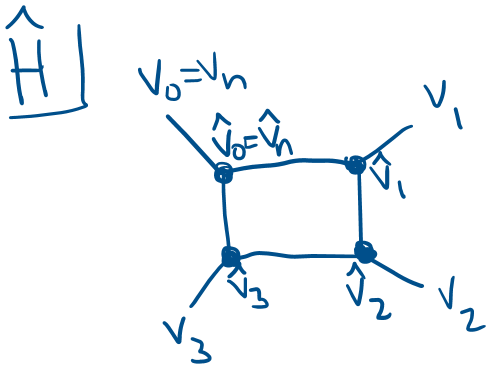
\includegraphics[width=.35\textwidth]{hdak.png}
    \caption{The graph $\hat H$.} \label{fig:hdak}
\end{figure}

Let the vertices on cycle $H$ be $v_0, v_1, \dots, v_n = v_0$.
Then the subproblem is defined in the following way: let $C[i, j, h(i), h(j)]$ be the minimum cost of only the part from $i$ to $j$ in $H$ (clockwise), where $\hat v_i$ is mapped to $h(i)$ and $\hat v_j$ is mapped to $h(j)$.
Here, $0 \le i < j \le n$ and all terminals must be mapped to itself.

If $j = i + 1$, then the cost is $b_i \cdot d_c(v_i, h(i)) + d_{ij} \cdot d_c(h(i), h(j)) + b_j \cdot d_c(v_j, h(j))$.
Here, $d_c(u, v)$ is the shortest path under cost function $c$ from $u$ to $v$ in $G$, i.e.\ buying each edge on the shortest path once.
It is considers the edge $\{\hat v_i, \hat v_j\}$ in the cycle in $\hat H$ and the two edges between these nodes and the corresponding terminals.
Because we required the capacities to be minimal, we know that there exist valid demands that utilize the full capacity.
Thus, we must buy these.

If $j$ is not $i+1$, we pick a node $\hat v_k$ with $i < k < j$ (for example, $k = i + 1$).
Then, $C[i, j, h(i), h(j)]$ is the minimum over all possible mappings $h(k) \in V_G$ of $C[i, k, h(i), h(k)] + C[k, j, h(k), h(j)] - b_k d(v_k, h(k))$.
Both parts consider the edge $(v_k, \hat v_k)$, so we should remove it once to obtain the correct answer.
See also Figure~\ref{fig:dp} for a sketch of the situation.

\begin{figure}
    \centering
    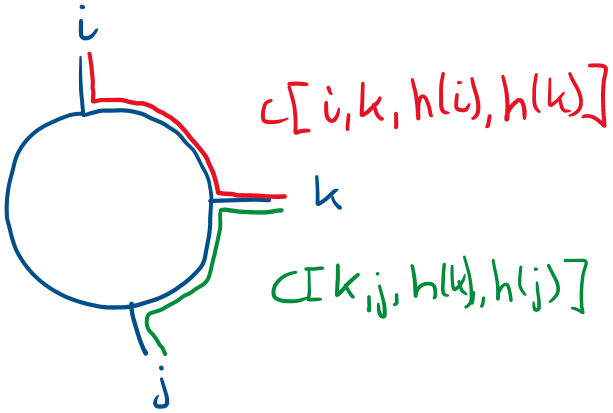
\includegraphics[width=.35\textwidth]{dp.png}
    \caption{Sketch of the situation for the dynamic program (in $\hat H$).} \label{fig:dp}
\end{figure}

This leads to the following recurrence:
\[
    C[i, j, h(i), h(j)] = \begin{cases}
                              0 &\text{if $i \ge j$} \\
                              b_i \cdot d_c(v_i, h(i)) + d_{ij} \cdot d_c(h(i), h(j)) + b_j \cdot d_c(v_j, h(j)) &\text{if $j = i+1$}\\
                              \displaystyle \min_{h(k) \in V_G} \{ C[i, k, h(i), h(k)] + C[k, j, h(k), h(j)] - b_k d(v_k, h(k)) \} &\text{otherwise}\\


    \end{cases}
\]

We can now determine all values by first determining the base cases, then all valid intervals of length two, then length three etc.
The last interval will go from $0$ to $n$ and this is the interval we are interested in.
However, notice that for a mapping $h(0)$ of $\hat v_0$, table entry $C[0, n, h(0), h(0)]$ will count the cost between $v_0$ and $h(0)$ twice.
Thus, the minimum cost is the minimum over all mappings $h(0)$ of $C[0, n, h(0), h(0)] - b_0 d(v_0, h(0))$.
The actual mappings can be obtained by searching the table backwards.

%\subsection{Experiments}
%Experiments with integrality gap.

\subsection{Proving optimality of the hubbing algorithm in the cycle case}
In this section, we explore an approach to generalize the proof in \cite{bosman2017exploring} that the hubbing programming algorithm is optimal when $H$ is a cycle and $b$, $d$ unit, to our setting where $b$ and $d$ are arbitrary.

The original proof first shows that there is always an optimal solution with a certain nice structure, but is not quite yet a hubbing solution.
A last, rather non-trivial step of the proof shows that this structure can in fact be transformed to a hubbing solution.


To obtain this first structured optimal solution, it is first shown that we can restrict ourselves solutions of the compact MIP formulation where the (originally dual) variable from the row subproblem is integral.
We now show that we can extend this integrality assumption to our case as well, in particular, we will show that we can restrict to solutions where $\omega$ and $\psi$ in our compact formulation are integral.
We are now slightly adapting the notation from the previous sections to match with \cite{bosman2017exploring}: for an edge $e = \{u, v\}$ we now write $\omega_i(e)$ and $\psi_{ij}(e)$ instead of $\omega_i^{uv}$ and $\psi_{ij}^{uv}$.

\subsubsection{Rephrashed version of the problem}
In order to show this, we first write an expression for the minimum capacity we are required to buy for each edge, if we consider the routing template to be given.
The required capacity for an edge $e \in E(G)$ becomes
\[
    x(e) = \max_{D \in \mathcal H^\text{cap}(b, d)} \sum_{\substack{ij \in \binom W 2 :\\e \in P_{ij}}} D_{ij}.
\]
The resulting solution has cost $\sum_e c(e) x(e)$, and this we wish to minimize.

We can also formulate the dual version of the above, from which we obtain a convenient rephrased version of the problem.
The dual is formulated as
\[
    \begin{split}
        x(e) = \min \quad & \sum_{i \in W} b_i \omega_i(e) + \sum_{ij \in \binom W 2} d_{ij} \psi_{ij}(e) \\
        \text{s.t.}\quad & \omega_i(e) + \omega_j(e) + \psi_{ij}(e) \ge 1 \qquad \forall_{ij \in E(H) : e \in P_{ij}} \\
        & \omega_i(e),\ \psi_{ij}(e) \ge 0.
    \end{split}
\]
We then rephrase the problem as follows.
Each terminal $i$ `buys' a capacity vector $\omega_i$, and each connection $ij$ `buys' a capacity vector $\psi_{ij}$ (indexed by the edges $e \in E$ of $G$), with the property that $\{ e \in E : \omega_i(e) + \omega_j(e) + \psi_{ij}(e) \ge 1 \}$ contains an $i$--$j$-path, for each connection $ij \in E(H)$.
The goal is to minimize the total cost
\[
    \sum_{e \in E} c(e) u(e) = \sum_{i} b_i c(\omega_i) + \sum_{ij} d_{ij} c(\psi_{ij}),
\]
where $c(\omega_i) = \sum_{e \in E} c(e) \omega_i(e)$ and $c(\psi_{ij}) = \sum_{e \in E} c(e) \psi_{ij}(e)$ (one can verify the total cost expression by substituting the dual objective for $u(e)$, merging the ``min''s, and re-arranging the summations).

\subsubsection{Integral solutions}
We will show that Lemma~4 of \cite{bosman2017exploring} generalizes to our case, i.e.\ that we can restrict to integral capacity vectors $(\boldsymbol \omega, \boldsymbol \psi)$.
\begin{proof}
    First, note that in any optimal, possibly fractional, solution, we have that $0 \le \omega_i, \psi_{ij} \le 1$, by the nature of the dual formulation.
    Hence, if the solution is integral, we know that the capacity vectors are binary.
    It is convenient to express the solution as a collection of edge sets (which we denote with a capital letter) $\boldsymbol \Omega = (\Omega_i)$ and $\boldsymbol \Psi = (\Psi_{ij})$, where $\Omega_i = \{ e : \omega_i(e) = 1 \}$ and $\Psi_{ij} = \{ e : \psi_{ij}(e) = 1 \}$, i.e.\ the edges that each terminal/connection buys.

    We now assume that $H$ is a cycle, and show that there always exists an integral optimum solution to the capped hose problem.
    Notice that $u(e)$ is phrased as a fractional $d$-capacitated $b$-matching problem on $H$, which has an integral optimal solution if $H$ is bipartite (since the constraint matrix is the incidence matrix of $H$, which is totally unimodular, see also \cite{schrijver2003combinatorial} Theorem~21.8).
    Hence, if $H$ is an even cycle, it is bipartite and we are done.

    Now, consider the case when $H$ is an odd cycle.
    Since any strict subgraph of a cycle is bipartite, the only case where we do not have an integral optimal solution is when $u(e)$ corresponds to the dual $d$-capacitated $b$-matching problem on the complete cycle.
    This only happens if the routing path between \emph{every} pair of neighbors uses the edge.

    So suppose $e = \{u, v\}$ is used on every routing path $P_{ij} \in \mathcal P$.
    Let $(\boldsymbol \omega, \boldsymbol \psi)$ a (possibly fractional) dual solution, with corresponding primal solution $D$.
    We first assume that this solution saturates $b$, i.e.\ the optimal primal solution $D$ satisfies
    \[
        D_{i-1,i} + D_{i,i+1} = b_i
    \]
    for all $i \in W$.
    We claim that the integral solution $(\boldsymbol Y, \boldsymbol Z)$, given by:
    \begin{itemize}
        \item taking $Y_i$ to be the set of edges of a shortest $i$--$v$-path (for all terminals $i$),
        \item taking $Z_{ij} = \varnothing$,
    \end{itemize}
    costs no more than $(\boldsymbol \omega, \boldsymbol \psi)$.

    The following closely resembles the arguments from \cite{bosman2017exploring}.
    We let $D$ be the traffic matrix from the primal solution.
    If we now route $D$ according to $(\boldsymbol \omega, \boldsymbol \psi)$, the flow between $i$ and $i+1$ can be split into flow between $i$--$v$ and flow between $v$--$(i+1)$, since every routing path passes through $e$, and thus through $v$.

    So $D$ induces a $i$--$v$ flow for each $i \in W$ of at least $b_i$, following directly from the fact that $b$ is saturated.
    So $(\boldsymbol \omega, \boldsymbol \psi)$ has sufficient capacity to route $b_i$ unit of flow from each $i \in W$ simultaneously.
    This costs at least as much as buying $b_i$ of every edge on a shortest path from terminal $i$ to $v$, for all terminals.
    The latter is exactly the cost of the integral solution $(\boldsymbol Y, \boldsymbol Z)$, proving the claim.

    We are left with the case where $\boldsymbol b$ is not saturated.
    We show that this is equivalent with a fractional capacitated $b$-matching problem on a path, which is bipartite and therefore shows that the solution is integral.

    As $\boldsymbol b$ is not saturated, there exists a terminal $i \in W$ such that
    \[
        D_{i-1,i} + D_{i,i+1} < b_i.
    \]
    By complementary slackness, we must have $\omega_i(e) = 0$.
    Construct now a new (fractional) $d'$-capacitated $b'$-matching problem on the graph $H'$ obtained from $H$ after `splitting' vertex $i$ (see Figure~\ref{fig:split}, which is much clearer than the formal definition in the next sentence).
    Thus, $H$ has vertex set $W\setminus \{i\} \cup \{i', i''\}$ and edge set $E(H') = E(H) \setminus \{ \{i-1,i\}, \{i, i+1\} \} \cup \{ \{i-1, i'\}, \{i'', i+1\} \}$.
    Set the connection capacities $d'_{i-1,i'} = d_{i-1,i}$, $d'_{i'',i+1} = d_{i,i+1}$ and $d'_{u,v} = d_{u,v}$ for pairs $uv$ not involving $i$, $i'$ or $i''$.
    Set the terminal capacities $b'_{i'} = b'_{i''} = \infty$ and $b'_j = b_j$ otherwise.

    \begin{figure}
        \centering
        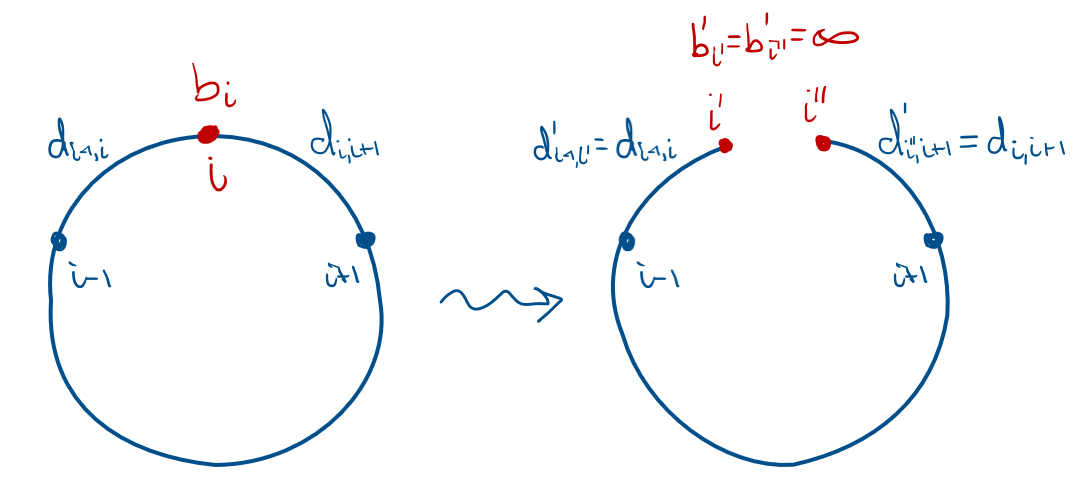
\includegraphics[width=.65\textwidth]{split}
        \caption{Construction of a new bipartite instance.} \label{fig:split}
    \end{figure}

    Note that the $(\boldsymbol \omega, \boldsymbol \psi)$ corresponds to a feasible dual solution $(\boldsymbol \omega', \boldsymbol \psi')$ in the constructed problem for $H'$, by setting $\omega'_{i'} = \omega'_{i''} = 0$.
    Note that the cost for both solutions are equal.
    We now argue that the constructed solution is optimal.
    We first observe that any optimal solution must have $\omega'_{i'} = \omega'_{i''} = 0$, as otherwise the objective becomes $\infty$.
    If there would exist a different solution with strictly smaller objective, this would correspond to a solution in the original problem with the same (strictly smaller) objective, contradicting optimality of $(\boldsymbol \omega, \boldsymbol \psi)$.
    Hence, $(\boldsymbol \omega', \boldsymbol \psi')$ is integral as $H'$ is bipartite, and hence $(\boldsymbol \omega, \boldsymbol \psi)$ is integral as well.
\end{proof}

\subsubsection{Integrality gap instances}
The proof is useful as an extension of Lemma~4 from \cite{bosman2017exploring}.
For the compact MIP formulation above, this proof shows that if we can assume $f$ is integral, then this implies that $\omega$ and $\psi$ are also integral.
Also the reverse implication holds, as for fixed integer $\omega$ and $\psi$ the problem reduces to a multicommodity flow problem with integer capacities.
This does not mean, however, that the whole formulation is integral.
Indeed, there exist instances for which an integrality gap is present, even for the case where $b$ and $d$ are unit.
These instances are the natural extension of integrality gap instances identified for the VPN problem and presented in \cite{goyal2013vpn}.
The largest integrality gap we found is using the graph with $4$ terminals in Figure~\ref{fig:gap4}, where the cycle is defined by unit $b$ and $d$.
This instance gives an integrality gap of $9/8$, which is the same integrality gap as found for the VPN problem.
To the best of our knowledge, integrality gap instanced for the capped hose problem where $H$ is a cycle have not been identified before.

\begin{figure}
    \centering
    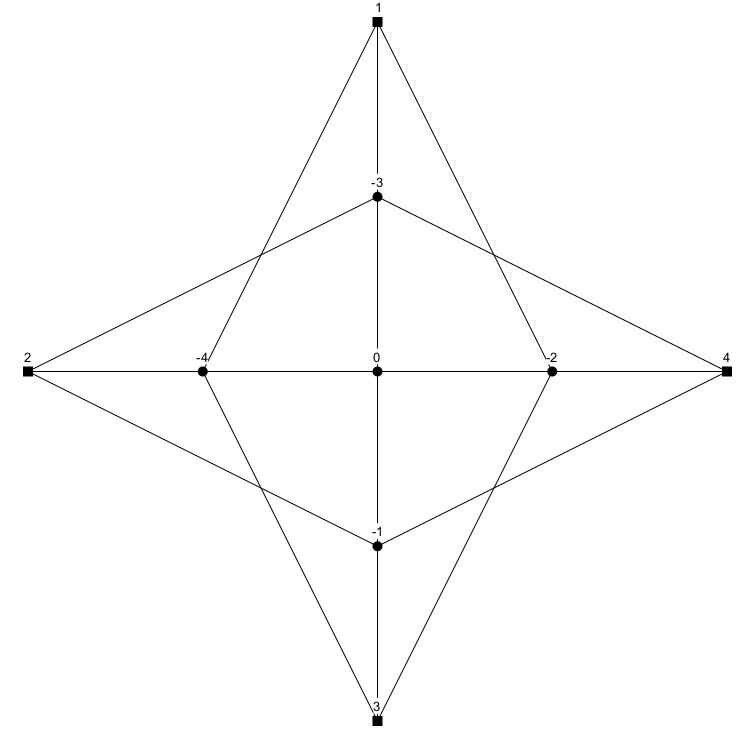
\includegraphics[width=.45\textwidth]{gap4}
    \caption{Integrality gap of $9/8$.} \label{fig:gap4}
\end{figure}

\subsubsection{Generalizing further}
It remains open whether it is possible to generalize the rest of the proof any further, as there are some challenges still to overcome there.
In short, the setup in definition~5 in \cite{bosman2017exploring} generalizes---maybe quite surprisingly---almost directly.
The partition of the mentioned feasible solution $\bar{\boldsymbol X}$ into sets $\bar{\boldsymbol X}_i$ and $\bar{\boldsymbol X}_{i,i+1}$ will intuitively correspond to the edges that are bought by terminals and connections, respectively.
We expect however that problems will arise in the proofs of lemma~11 and lemma~13, as here a solution $\bar{\boldsymbol X}$ is transformed into a different solution $\bar{\boldsymbol Y}$ by possibly switching edges from being bought by a terminal to being bought by a connection (or vice versa).
We make this clear with the following intuitive but very informal argument.
When being careful how many edges are switched, the cost of the resulting solution will not increase in the case where $b$ and $d$ are unit: you pay the same price for capacity regardless of whether the edge is bought by a terminal or a connection.
For arbitrary $b$ and $d$ this is no longer the case, and switching `buyers' of edge capacity might increase the total cost of the solution.
Luckily, the requirement that $b$ and $d$ are minimal gives some restriction on how much the cost can increase, but it is not immediately clear that the proofs of lemma~11 and lemma~13 will generalize.


    \section{Conclusion}
    % TODO

    \bibliographystyle{plain}
    \bibliography{references}

    \clearpage
    \appendix
    \section{Proving the generalized VPN conjecture on ring networks} \label{app:proof}
When we assume there always exists an optimal hubbing solution for the generalized VPN problem that is also a tree solution, one can try to prove the generalized VPN conjecture with the same ideas as presented in \cite{grandoni2008short}.
However, as stated in Section~\ref{subsec:genvpn:rings}, this assumption can in general not be made.
In any case, our efforts of generalizing the proof under the assumption are layed out in this section.
The ideas here are in no way complete, and some (parts of) proofs are missing for a number of introduced theorems and lemmas.
In particular, Claim~4 from \cite{grandoni2008short} is problematic, and this fails to let the final inductive argument work.

Some background of what steps we are taking is identical to what is described in \cite{grandoni2008short} and we will omit these details.
We focus on showing the differences that are necessary in the proof to adapt to the generalized VPN problem setting.
We use the same notation as used in the aforementioned paper, except where the generalized VPN problem differs from the VPN problem.

For the remainder, we restrict ourselves to instances where $T$ is a \emph{two-union star}, that is, a tree formed by connecting the centers $r_1,\ r_2$ of two star graphs.
We will call this edge $r = \set{r_1, r_2}$ and refer to it as the \emph{bridge} of $T$.

\subsection{Preliminaries}
A number of assumptions are made in \cite{grandoni2008short}, the most important being that we can assume the capacities $b \equiv 1$.
We suspect this does not quite generalize to our case, but we can state the following:

\begin{fact}
    We may assume $b_f = 1$ when $f \neq r$.
\end{fact}
Using the same motivation as in \cite{grandoni2008short}, if the capacity $b_{iu}$ for a terminal $i \in W$ is not unit, construct a new instance with new terminals $i_1, \dots, i_{b_{iu}}$, connected to the site of $i$ in $G$, with edge cost $0$.
Set the capacities of the incident edges in $T$ to unit.
Note that this instance is equivalent, but may change the topology of the graph.

An alternative construction is argued in \cite{grandoni2008short} to keep the topology a ring and we refer to this paper for the details.

\begin{fact}
    We can assume $b$ to be integral.
\end{fact}
This is motivated by scaling by a sufficiently large factor.

\subsection{Pyramidal routing problem}
To goal is to show that there exists an optimal solution to the generalized VPN problem that is a tree solution (or, equivalently, there exists a tree solution to the generalized VPN problem that is optimal).
Consider an optimal tree solution $(\set{P_{ij}}, x)$ to a generalized VPN instance $(G, c, W, T, b)$, with $|W| = k$ and $T$ a two-union star with the unit capacity assumption as above.
Let $\mathcal P_i$ be as in \cite{grandoni2008short} for a fixed $i \in W$.
We define
\[
    \xi(e, \mathcal P_i) \coloneqq \min\set{\alpha(e, \mathcal P_i),\ \beta(e, \mathcal P_i)} + \min\set{n(e, \mathcal P_i) - \alpha(e, \mathcal P_i),\ k - n(e, \mathcal P_i) - \beta(e, \mathcal P_i)}
\]
where
\begin{gather*}
    n(e, \mathcal P_i) \coloneqq |\set{j \in W \setminus \set{i} : e \in P_{ij}}|,\\
    \alpha(e, \mathcal P_i) \coloneqq |\set{j \in W \setminus \set{i} : e \in P_{ij},\ r \in \pi_T(i, j)}|,\\
    \beta(e, \mathcal P_i) \coloneqq |\set{j \in W \setminus \set{i} : e \not\in P_{ij},\ r \not\in \pi_T(i, j)}|,
\end{gather*}
that is, $\alpha(e, \mathcal P_i)$ is the number of paths in $\mathcal P_i$ containing $e$, \emph{while simultaneously the path in the demand tree between $i$ and $j$ crosses the bridge}.
In our setting, we have a different expression for the \emph{required} capacity of edge $e$:
\[
    x(e) = \xi(e, \mathcal P_i) + \min\Big\{b(r),\ n(e, \mathcal P_i) - \xi(e, \mathcal P_i),\ k - n(e, \mathcal P_i) -  \xi(e, \mathcal P_i)\Big\}.
\]
We can now formulate the generalized Pyramidal Routing (\emph{genPR}) problem with instance $(G, c, W, T, b, i)$ as to minimize $\sum_{e \in E_G} c(e) y(e, \mathcal P_i)$ over all $\mathcal P_i$ (for an arbitrary fixed $i \in W$), where we define
\[
    y(e, \mathcal P_i) = \xi(e, \mathcal P_i) + \min\Big\{b(r),\ n(e, \mathcal P_i) - \xi(e, \mathcal P_i),\ k - n(e, \mathcal P_i) -  \xi(e, \mathcal P_i)\Big\}.
\]

We now formulate our version of Conjecture~2 (as in \cite{grandoni2008short}).
\renewcommand\theconjecture{2}
\begin{conjecture}[The \emph{genPR} conjecture]
    For each \emph{genPR} instance $(G, C, W, i, T, b)$ there exists an optimal solution which is a tree solution.
\end{conjecture}

We now show our version of Theorem~1 (having the same formulation as in \cite{grandoni2008short}), using the equivalent of Lemma~3, Claim~1, and Claim~2.

\renewcommand\thelemma{3}
\begin{lemma}
    Consider an generalized VPN instance $(G, c, W, T, b)$ with $T$ a two-union star with bridge $r$, $b(f) = 1$ for $f \neq r$, and some feasible solution $(\set{P_{ij}}, u)$.
    There exists a terminal $i \in W$ such that $\sum_{e \in E_G} c(e) u(e) \ge \sum_{e \in E_G} c(e) y(e, \mathcal P_i)$, where $\mathcal P_i = \set{P_{ij} : j \in W \setminus \set{i}}$.
\end{lemma}
\begin{proof}
    Fix an edge $e \in E_G$.
    We define the same traffic matrix $D^e = (d^e_{ij})_{i,j \in W}$ as in \cite{grandoni2008short},
    \[
        d^e_{ij} = \begin{cases}
                       \frac 1 k \left( \frac{y(e, \mathcal P_i)}{n(e, \mathcal P_i)} + \frac{y(e, \mathcal P_j)}{n(e, \mathcal P_j)} \right) & \text{if $e \in P_{ij}$,} \\
                       0 & \text{otherwise.}
        \end{cases}
    \]

    Now, the proof of Claim~1 is slightly different, as our universe is described by a different set of inequalities.

    \renewcommand\theclaim{1}
    \begin{claim}
        $D^e \in \mathcal U_T$, that is
        \[
            \sum_{\substack{ij \in \binom{W}{2}:\\f \in \pi_T(i,j)}} d^e_{ij} \le b(f)
        \]
        for all $f \in E_T$.
    \end{claim}
    \begin{proof}
        We consider two cases:
        \begin{itemize}
            \item $f \neq r$, hence we can write $f = f_i$, where $f_i \in E_T$ is the edge incident some terminal $i \in W$.
            Now note that we can write
            \[
                \sum_{\substack{\ell j \in \binom{W}{2}:\\f_i \in \pi_T(\ell,j)}} d^e_{\ell j} = \sum_{j \in W \setminus \set{i}} d^e_{ij}
            \]
            as $f_i$ is exactly in all paths from/to $i$ in the tree, as it is the edge incident to $i$.
            The rest of this case follows the same steps as the proof in \cite{grandoni2008short}:
            \[
                \begin{split}
                    \sum_{\substack{\ell j \in \binom{W}{2}:\\f_i \in \pi_T(\ell,j)}} d^e_{\ell j} &= \sum_{j \in W \setminus \set{i}} d^e_{ij} \\
                    &= \frac 1 k \sum_{\substack{j \in W \setminus \set{i}:\\ e \in P_{ij}}} \left( \frac{y(e, \mathcal P_i)}{n(e, \mathcal P_i)} + \frac{y(e, \mathcal P_j)}{n(e, \mathcal P_j)} \right) \\
                    &\le \frac 1 k \sum_{\substack{j \in W \setminus \set{i}:\\ e \in P_{ij}}} \left( \frac{k - n(e, \mathcal P_i)}{n(e, \mathcal P_i)} + \frac{n(e, \mathcal P_j)}{n(e, \mathcal P_j)} \right) \\
                    &= \frac{1}{n(e, \mathcal P_i)} \sum_{\substack{j \in W \setminus \set{i}:\\ e \in P_{ij}}} 1 \\
                    &= 1 \\
                    &= b(f_i).
                \end{split}
            \]

            \item $f = r$.
            We have not been able, with the current definition of $y$ and $D^e$, to make this work.
            However, we reduced it to a more accessible form.
            In the third line, we exchange the order of the two sums and use the symmetry of $\pi_T(i, j)$ and $P_{ij}$.
            \[
                \begin{split}
                    \sum_{\substack{ij \in \binom{W}{2},\\r \in \pi_T(i,j)}} d^e_{ij} &= \frac 1 2 \sum_{i \in W} \sum_{\substack{j \in W \setminus \set{i}:\\r \in \pi_T(i,j)}} d^e_{ij} \\
                    &= \frac{1}{2k} \sum_{i \in W} \sum_{\substack{j \in W \setminus \set{i}:\\r \in \pi_T(i,j),\\e \in P_{ij}}} \frac{y(e, \mathcal P_i)}{n(e, \mathcal P_i)} + \frac{1}{2k} \sum_{i \in W} \sum_{\substack{j \in W \setminus \set{i}:\\r \in \pi_T(i,j),\\e \in P_{ij}}} \frac{y(e, \mathcal P_j)}{n(e, \mathcal P_j)} \\
                    &= \frac{1}{2k} \sum_{i \in W} \sum_{\substack{j \in W \setminus \set{i}:\\r \in \pi_T(i,j),\\e \in P_{ij}}} \frac{y(e, \mathcal P_i)}{n(e, \mathcal P_i)} + \frac{1}{2k} \sum_{j \in W} \sum_{\substack{i \in W \setminus \set{j}:\\r \in \pi_T(j,i),\\e \in P_{ji}}} \frac{y(e, \mathcal P_j)}{n(e, \mathcal P_j)} \\
                    &= \frac{1}{k} \sum_{i \in W} \sum_{\substack{j \in W \setminus \set{i}:\\r \in \pi_T(i,j),\\e \in P_{ij}}} \frac{y(e, \mathcal P_i)}{n(e, \mathcal P_i)} \\
                    &= \frac{1}{k} \sum_{\substack{i \in W:\\n(e, \mathcal P_i) > 0}} \left( \alpha(e, \mathcal P_i) \frac{y(e, \mathcal P_i)}{n(e, \mathcal P_i)} \right) \\
                    &\ \vdots \text{\ (missing)}\\
                    &\le b(r).
                \end{split}
            \] \qedhere
        \end{itemize}

    \end{proof}
    The remainder of the proof of Lemma~3 (and Claim~2) is exactly the same as in \cite{grandoni2008short}, as the definition of $D^e$ is exactly the same, and the definition of $y(e, \mathcal P_i)$ itself is not used.
\end{proof}

From this follows (our version of) Theorem~1, stating that on ring networks, if there exists an optimal tree solution for the \emph{genPR} problem, that also an optimal tree solution exists for the generalized VPN problem.

Now, what remains to show is that indeed an optimal tree solution exists for the \emph{genPR} problem when $G$ is a ring.
If we follow the structure of the proof in \cite{grandoni2008short}, not first that Claim~3 also holds for our case.
However, Claim~4 does not hold: it might be that $y(e, \mathcal P_i) = y(f, \mathcal P_i) = b(r)$ (in the second case of the definition of $y$).

We are not sure that the counterexample for Claim~4 is actually problematic, or how to circumvent this issue in the last step of completing the argument.


\end{document}
